\documentclass[15pt]{beamer}
  
\newcommand\blfootnote[1]{%
  \begingroup
  \renewcommand\thefootnote{}\footnote{#1}%
  \addtocounter{footnote}{-1}%
  \endgroup
  }
%
% Choose how your presentation looks.
%
% For more themes, color themes and font themes, see:
% http://deic.uab.es/~iblanes/beamer_gallery/index_by_theme.html
%
\mode<presentation>
{
  \usetheme{default}      % or try Darmstadt, Madrid, Warsaw, ...
  \usecolortheme{default} % or try albatross, beaver, crane, ...
  \usefonttheme{default}  % or try serif, structurebold, ...
  \setbeamertemplate{navigation symbols}{}
  \setbeamertemplate{caption}[numbered]

} 

\usepackage[english]{babel}
\usepackage[utf8x]{inputenc}
\usepackage[absolute,overlay]{textpos}
\usepackage{amsmath}
\usepackage{lipsum}


\title[Your Short Title]{Modifying interactions to switch steady states}
\author{Jean Carlson group}
\institute{UCSB}
\date{October 12, 2018}

\begin{document}

\begin{frame}
  \titlepage
\end{frame}

% Uncomment these lines for an automatically generated outline.
%\begin{frame}{Outline}
%  \tableofcontents
%\end{frame}

\section{Introduction}

%%%%%%%%%%%%%%%%%%%%slide 1
\begin{frame}{Project Goal}
\begin{columns}
\column{0.5\textwidth}
\begin{itemize}
	\item Move separatrix to switch steady states
	\item Changing interaction matrix using SSR as a guide
\end{itemize}
 
\column{0.5\textwidth}
	\begin{textblock*}{6.8cm}(6.5cm,3cm) % {block width} (coords)
	 \includegraphics[width=0.9\textwidth]{attractor_network_v3_w_arrow}\\[-1ex]
	 {\tiny }
	\end{textblock*}
\end{columns}
\end{frame}

%%%%%%%%%%%%%%%%%%%%slide 1.5
\begin{frame}{Bifurcation Analysis}
\begin{columns}
\column{0.5\textwidth}
\begin{itemize}
	\item Separatrix moves with the third steady state
	\item Originally in upper right region
	\item going towards upper left
\end{itemize}
\column{0.5\textwidth}
	\begin{textblock*}{7.6cm}(5.5cm,1cm) % {block width} (coords)
	 \includegraphics[width=0.9\textwidth]{bifurcation}
	 {\small
	  Black dots shows stable steady states, and \\hollow dots shows unstable steady states}
	\end{textblock*}
\end{columns}
\end{frame}

\section{Result}
%%%%%%%%%%%%%%%%%%%%slide 2
\begin{frame}{Change in 2-D matrix}
\begin{columns}
\column{0.5\textwidth}
\begin{textblock*}{7cm}(0cm,1.3cm) % {block width} (coords)
	 \includegraphics[width=0.9\textwidth]{phase_space}
	\end{textblock*}
\column{0.5\textwidth}
	\begin{textblock*}{7.3cm}(6.2cm,1cm) % {block width} (coords)
	 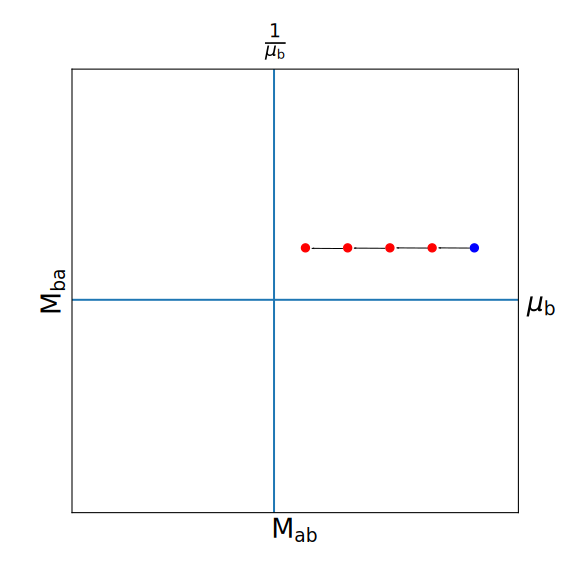
\includegraphics[width=0.9\textwidth]{parameter_space}
	\end{textblock*}
\end{columns}
\begin{textblock*}{6cm}(1.4cm,7.6cm) % {block width} (coords)
Microbial Phase Space
\end{textblock*}
\begin{textblock*}{6cm}(8.2cm,7.6cm) % {block width} (coords)
Parameter Space
\end{textblock*}
\end{frame}

%%%%%%%%%%%%%%%%%%%%slide 3
\begin{frame}{Change in K}
\begin{columns}
\column{0.45\textwidth}
\begin{align*}
M_{ab} &= \vec{y_a}^T K \vec{y_b}\\
	   &= \sum_{i=1,j=1}^{11,11} \alpha_{ij}K_{ij}
\end{align*}

\begin{itemize}
	\item 121 coefficients
	\item Most are 0
	\item $M_{ab}$ most sensitive to change in $k_{ij}$ with the largest $\alpha_{ij}$ coefficient
\end{itemize}

\column{0.45\textwidth}
	\begin{textblock*}{8cm}(5.5cm,2cm) % {block width} (coords)
	 \includegraphics[width=0.9\textwidth]{hist}
	\end{textblock*}
\end{columns}
\end{frame}

%%%%%%%%%%%%%%%%%%%%slide 4
\begin{frame}{Projection of $\Delta K$ back to 2-D}
\begin{columns}
\column{0.5\textwidth}
\begin{itemize}
	\item Change in K could change $M_{ba}$
	\item In this case $M_{ba}$ does not change
	\item Check if SSR coefficients for $M_{ba}$ and $M_{ab}$ are orthogonal
\end{itemize}
 
\column{0.5\textwidth}
	\begin{textblock*}{7.3cm}(6.2cm,2cm) % {block width} (coords)
	 \includegraphics[width=0.9\textwidth]{projection_delta_K}\\[-1ex]
	 {\tiny }
	\end{textblock*}
\end{columns}
\end{frame}

%%%%%%%%%%%%%%%%%%%%slide 5
\begin{frame}{Projection of $\Delta K$ back to 2-D}
\begin{columns}
\column{0.45\textwidth}
\begin{align*}
M_{ab} &= \sum_{i=1,j=1}^{11,11} \alpha_{ij}K_{ij}\\
M_{ba} &= \sum_{i=1,j=1}^{11,11} \beta_{ij}K_{ij}\\
\gamma_{ij} &= \alpha_{ij}\beta_{ij}
\end{align*}

\begin{itemize}
	\item check the value of $\gamma_{ij}$
	\item $\alpha_{ij}$ and $\beta_{ij}$ are nearly orthogonal, with one exception 
\end{itemize}
	
\column{0.45\textwidth}
	\begin{textblock*}{8cm}(5.5cm,2cm) % {block width} (coords)
	 \includegraphics[width=0.9\textwidth]{parameter_check}
	\end{textblock*}
\end{columns}
\end{frame}

%%%%%%%%%%%%%%%%%%%%slide 6
\begin{frame}{Separatrix in 11-D}
\begin{columns}
\column{0.45\textwidth}
\begin{itemize}
	\item Numerically calculate separatrix by simulation
	\item Generate a separatrix curve 
\end{itemize}
	
\column{0.45\textwidth}
	\begin{textblock*}{7.6cm}(5.7cm,2cm) % {block width} (coords)
	 \includegraphics[width=0.9\textwidth]{gLV_phases_N_23_plot}
	\end{textblock*}
\end{columns}
\end{frame}

%%%%%%%%%%%%%%%%%%%%slide 7
\begin{frame}{Change in 11-D separatrix}
\begin{columns}
\column{0.45\textwidth}
\begin{itemize}
	\item 11-D simulation after change in K
	\item Half of the plane does not go to either steady states
\end{itemize}
	
\column{0.45\textwidth}
	\begin{textblock*}{7.6cm}(5.7cm,2cm) % {block width} (coords)
	 \includegraphics[width=0.9\textwidth]{gLV_phases_N_change23_plot}
	\end{textblock*}
\end{columns}
\end{frame}

%%%%%%%%%%%%%%%%%%%%slide 7
\begin{frame}{Change in 11-D separatrix}
\begin{columns}
\column{0.45\textwidth}
\begin{itemize}
	\item the separatrix changes with small changes of K
	\item similar to change in M
\end{itemize}
	
\column{0.45\textwidth}
	\begin{textblock*}{8cm}(6cm,1cm) % {block width} (coords)
	 \includegraphics[width=0.9\textwidth]{delta_K_separatrix}
	\end{textblock*}
\end{columns}
\end{frame}

%%%%%%%%%%%%%%%%%%%%slide 7.5
\begin{frame}{Change in 11-D separatrix}
\begin{columns}
\column{0.5\textwidth}
\begin{textblock*}{7.1cm}(0cm,1.6cm) % {block width} (coords)
	 \includegraphics[width=0.9\textwidth]{phase_space}
	\end{textblock*}
	
\column{0.45\textwidth}
	\begin{textblock*}{7.8cm}(6.2cm,1cm) % {block width} (coords)
	 \includegraphics[width=0.9\textwidth]{delta_K_separatrix}
	\end{textblock*}
\end{columns}
\end{frame}

%%%%%%%%%%%%%%%%%%%%slide 8
\begin{frame}{Future steps}
\begin{itemize}
	\item Apply the procedure to other pairs of steady states
	\item Make the change in interaction matrix temporary
	\item Other complex systems
\end{itemize}
\end{frame}

\end{document}
